\documentclass[11pt,a4paper]{article}

\usepackage[utf8]{inputenc}
\usepackage[T1]{fontenc}
\usepackage[english]{babel}
\usepackage[a4paper,margin=2.4cm]{geometry}

\usepackage{amsmath, amssymb, amsthm}
\usepackage{mathtools}
\usepackage{stmaryrd}
\usepackage{booktabs}
\usepackage{tabularx}
\usepackage{array}
\usepackage{caption}
\usepackage{subcaption}
\usepackage{float}
\usepackage{enumitem}
\usepackage{microtype}
\usepackage{xcolor}
\usepackage{listings}
\usepackage{fancyhdr}
\usepackage{titlesec}
\usepackage{graphicx}
\usepackage{tikz}
\usetikzlibrary{positioning, arrows.meta, fit, backgrounds, calc, shapes.geometric}
\usepackage[hidelinks]{hyperref}

%  ---  Palette shared with the companion reports  ---
\definecolor{ink}{RGB}{26,30,36}
\definecolor{slate}{RGB}{92,101,112}
\definecolor{mist}{RGB}{233,235,238}
\definecolor{rulegrey}{RGB}{188,194,201}
\definecolor{steel}{RGB}{47,72,102}
\definecolor{steellight}{RGB}{124,146,172}
\definecolor{signal}{RGB}{160,32,45}
\definecolor{conciergec}{RGB}{40,90,180}
\definecolor{cleanerc}{RGB}{40,140,80}
\definecolor{knows}{RGB}{26,140,70}

\hypersetup{
    colorlinks=true,
    linkcolor=steel,
    citecolor=steel,
    urlcolor=steel,
    pdftitle={Knowledge No Robot Holds Alone},
    pdfauthor={Haniel Ulises},
}

\color{ink}

\setlength{\headheight}{22pt}
\pagestyle{fancy}
\fancyhf{}
\fancyhead[L]{\small\textcolor{slate}{\itshape Knowledge No Robot Holds Alone}}
\fancyhead[R]{\small\textcolor{slate}{\thepage}}
\renewcommand{\headrulewidth}{0.4pt}
\renewcommand{\headrule}{\hbox to\headwidth{\color{rulegrey}\leaders\hrule height \headrulewidth\hfill}}

\titleformat{\section}{\normalfont\large\bfseries\color{ink}}{\thesection}{0.7em}{}
\titleformat{\subsection}{\normalfont\normalsize\bfseries\color{ink}}{\thesubsection}{0.7em}{}
\titleformat{\paragraph}[runin]{\normalfont\bfseries\color{slate}}{}{0em}{}[.]

\captionsetup{font=small, labelfont={bf,color=slate}, textfont=footnotesize}

\theoremstyle{definition}
\newtheorem{definition}{Definition}
\newtheorem{proposition}{Proposition}
\newtheorem{lemma}{Lemma}
\newtheorem{corollary}{Corollary}
\newtheorem{remark}{Remark}

\lstdefinestyle{sys}{
    backgroundcolor=\color{mist},
    basicstyle=\ttfamily\scriptsize\color{ink},
    keywordstyle=\color{steel}\bfseries,
    commentstyle=\color{slate}\itshape,
    stringstyle=\color{slate},
    morecomment=[l]{;},
    morekeywords={:types,:predicates,:objects,:agents,:goal,:init,:event,:action,:action-type,:observability-conditions,:precondition,:effects,:events,:relations,:designated,:conditions,:observability-types},
    frame=single,
    rulecolor=\color{rulegrey},
    framesep=5pt,
    xleftmargin=6pt,
    xrightmargin=0pt,
    breaklines=true,
    showstringspaces=false,
    columns=fullflexible,
    captionpos=b,
}
\lstset{style=sys}

%  ---  Notation  ---
\newcommand{\Mod}{\mathcal{M}}
\newcommand{\Ev}{\mathcal{E}}
\newcommand{\prd}{\otimes}
\newcommand{\Kw}[1]{\mathit{Kw}_{#1}}
\newcommand{\code}[1]{\texttt{\small #1}}
\newcommand{\pre}{\mathit{pre}}
\newcommand{\post}{\mathit{post}}
\newcommand{\safe}{\mathit{safe}}
\newcommand{\src}[1]{\mathit{source}_{#1}}
\newcommand{\fl}[1]{\mathit{floor}_{#1}}
\newcommand{\cl}[1]{\mathit{col}_{#1}}
\newcommand{\at}{\mathit{at}}

\begin{document}

\begin{titlepage}
\centering
\vspace*{2.4cm}
{\color{rulegrey}\rule{\textwidth}{0.8pt}}\\[0.9cm]
{\LARGE\bfseries Knowledge No Robot Holds Alone\par}
\vspace{0.5cm}
{\large\color{slate} Distributed Knowledge, Meeting Places, and an All-Clear\\
the Guest Could Read, in the Open-RMF Hotel\par}
\vspace{0.7cm}
{\color{rulegrey}\rule{\textwidth}{0.8pt}}\\[1.4cm]

{\large Haniel Ulises\par}
\vspace{0.3cm}
{\color{slate} Epistemic Robotics}\\
\vspace{0.15cm}
{\color{slate}\today}

\vfill
{\color{slate}\small
Water is coming through from one of four rooms of the Open-RMF hotel. The
cleaner, which cannot leave the ground floor, knows the column; the concierge
knows the floor; the porter, the only robot of the three that can ride a lift
with the valve key, knows neither; and a guest in the lobby must not learn the
room. Robots of different fleets can tell each other only where they meet, and
whoever else is there hears. The goal is that the leak be contained, that every
responder know that every responder knows it, and that the guest be unable to
rule out any room.

\vspace{0.6em}
We prove that the room is distributed knowledge of the cleaner and the
concierge and no agent's knowledge; that without a telling the porter must
open, on the deepest branch, every room but one; that after the porter has been
seen in a room, any public announcement that the leak is contained tells the
guest that room, however little it says; that a fleet whose only shared channel
is the public address has no policy for the goal, and a fleet with no shared
channel never stands down; and that the shortest policy has seven actions,
among them a ride back down that a rule keeping locations off the public
address would save. Aletheia returns that policy, and the policies of three
baseline fleets planned by the same planner; an exhaustive search settles the
two the planner cannot. All four were run in the stock hotel through ePlanSys
and Open-RMF, and only the epistemic fleet met the goal.}
\vspace{1.2cm}
\end{titlepage}

\tableofcontents
\newpage

%  ======================================================================
\section{Scope}
\label{sec:scope}

The hotel incident~\cite{ulises2026hotel} ran an epistemic policy in the same
building: two robots looked for a leak in one of two suites, the location was
found by inspection, and a guest who must not learn it ruled out the public
address. Every fact the mission needed was one robot's to observe. This report
takes a problem in which the fact the mission needs is no robot's: the room is
distributed knowledge of two robots of two fleets, the robot that must act on
it knows nothing, the channels between fleets are places in the building, and
the outsider's ignorance is a goal about what it can infer.

Six claims are advanced.

\begin{enumerate}[leftmargin=1.4em, itemsep=2pt]
  \item The room is distributed knowledge of the cleaner and the concierge and
        no agent's knowledge (Lemma~\ref{lem:dist}); before the containment the
        porter must hear both, or open, on its deepest branch, every room but one
        (Proposition~\ref{prop:pool}).
  \item Every model reachable in the domain is S5, positions are common
        knowledge, and an agent that is elsewhere learns no fact from an action
        (Lemmas~\ref{lem:s5}--\ref{lem:move}).
  \item After the porter has been seen in a room, any public announcement that
        the leak is contained tells the guest that room
        (Proposition~\ref{prop:allclear}). A rule keeping locations off the
        public address therefore fails at every leaf, and a fleet whose only
        channel between fleets is the public address has no policy
        (Corollaries~\ref{cor:filter} and~\ref{cor:paonly}).
  \item A fleet with no channel between fleets never reaches the stand-down
        (Proposition~\ref{prop:siloed}).
  \item The policy Aletheia returns meets the whole goal at every leaf, and no
        policy with fewer than seven actions does
        (Propositions~\ref{prop:policy} and~\ref{prop:depth}); for the goal
        without the secret, six suffice.
  \item Four fleets, planned by the same planner, were run in the stock
        Open-RMF hotel through ePlanSys, and each run's verdict on the whole goal,
        measured at the actual world, is the one the analysis gives
        (Section~\ref{sec:runs}).
\end{enumerate}

Three bounds are stated at the outset. No robot perceives: what the cleaner
says of the column, what the concierge says of the floor and what an opened
room shows are reported by the bridge to Open-RMF from the room the launch
names. No robot reasons for itself: who knows what is read from the model the
epistemic state maintains, evaluated at the actual world. The guest is an
agent of the model and a figure on the floor, and is taken to see every
robot's position.

%  ======================================================================
\section{Preliminaries}
\label{sec:prelim}

An epistemic model is $\Mod = (W, (R_a)_{a \in \mathcal{A}}, V, W_d)$ with
designated worlds $W_d$; $K_a\varphi$ holds at $w$ when $\varphi$ holds at every
world of $R_a(w)$, $\langle a\rangle\varphi$ is its dual, and for a group $G$,
$E_G\varphi = \bigwedge_{a \in G} K_a\varphi$, $C_G\varphi$ is $\varphi$ at
every world reachable from $w$ by one or more steps of $\bigcup_{a \in G} R_a$,
and the distributed knowledge $D_G\varphi$ is $\varphi$ at every world of
$\bigcap_{a \in G} R_a(w)$~\cite{fhmv1995}. An event model
$\Ev = (E, (Q_a), \pre, \post, E_d)$ is applied by the product
update~\cite{bms1998, vanditmarsch2007}: the worlds of $\Mod \prd \Ev$ are the
pairs $(w, e)$ with $\Mod, w \models \pre(e)$, $(w,e) \mathrel{R'_a} (v,f)$ iff
$w \mathrel{R_a} v$ and $e \mathrel{Q_a} f$, valuations follow $\post$, and the
designated pairs are those of $W_d \times E_d$. In EPDDL an agent's $Q_a$ is
chosen by an observability condition~\cite{ba2011}; plank and Aletheia evaluate
it once per state, at the designated worlds.

%  ======================================================================
\section{The domain}
\label{sec:domain}

\code{tools/hotel\_domain.py} writes the domain for $F$ floors and $K$ columns.
The hotel has $F = \{L2, L3\}$ and $K = \{\mathit{room1}, \mathit{room15}\}$, and
its rooms are $Z = F \times K$. The agents are $\mathcal{A} = \{c, t, p, g\}$,
the cleaner, the concierge, the porter and the guest, and the responders are
$R = \{c, t, p\}$. The atoms are $\fl{f}$, $\cl{k}$, $\src{z}$, $\safe$, and
$\at(a, x)$ for places $x \in X = \{\mathit{lobby}, \mathit{restaurant}\} \cup Z$.
Static facts give each robot's lanes, read off the three fleets' navigation
graphs: the cleaner moves between the lobby and the restaurant, the concierge
likewise, and the porter between the restaurant and every room, and between
rooms. The cleaner and the concierge start in the restaurant and the lobby, the
porter in the restaurant, the guest in the lobby.

\paragraph{The initial model}
$\Mod_0$ has one world per room, $W = Z$. At $w = (f, k)$ the valuation makes
$\fl{f}$, $\cl{k}$ and $\src{w}$ true and the other location atoms false;
positions and $\neg\safe$ are the same at every world. The relations are
\[
  (f,k) \mathrel{R_t} (f',k') \iff f = f', \qquad
  (f,k) \mathrel{R_c} (f',k') \iff k = k', \qquad
  R_p = R_g = W \times W,
\]
and $W_d = W$: the executor does not know the room either. The EPDDL states this
as common knowledge that exactly one floor and one column hold, that
$\src{(f,k)} \leftrightarrow \fl{f} \wedge \cl{k}$, that the concierge knows
whether each floor atom holds and the cleaner whether each column atom does,
and that no other agent knows either.

\begin{figure}[H]
\centering
\begin{tikzpicture}[w/.style={circle,draw=ink,thick,minimum size=12mm,inner sep=0pt,font=\small},
                    t/.style={conciergec, line width=1.6pt}, c/.style={cleanerc, line width=1.6pt}]
  \node[w, draw=signal, line width=1.6pt] (a) at (0,2) {$L3\cdot1$};
  \node[w] (b) at (3.4,2) {$L3\cdot15$};
  \node[w] (cc) at (0,0) {$L2\cdot1$};
  \node[w] (d) at (3.4,0) {$L2\cdot15$};
  \draw[t] (a) -- (b); \draw[t] (cc) -- (d);
  \draw[c] (a) -- (cc); \draw[c] (b) -- (d);
  \node[anchor=west, font=\small, text=conciergec] at (5,2.2) {concierge: same floor};
  \node[anchor=west, font=\small, text=cleanerc] at (5,1.6) {cleaner: same column};
  \node[anchor=west, font=\small, text=slate] at (5,1.0) {porter, guest: every pair};
  \node[anchor=west, font=\small, text=slate] at (5,0.4) {$R_c \cap R_t$ is the identity};
\end{tikzpicture}
\caption{The initial model. Loops are omitted and every world is designated;
the world ringed in red is the actual one in the runs.}
\label{fig:model}
\end{figure}

\begin{lemma}[Distributed, and nobody's]
\label{lem:dist}
For every $w \in W$, $\Mod_0, w \models D_{\{c,t\}}\,\src{w}$, and
$\Mod_0, w \not\models K_a\,\src{z}$ for every agent $a$ and room $z$. For a
group $G$ that does not contain both $c$ and $t$,
$\Mod_0, w \not\models D_G\,\src{z}$ for every $z$.
\end{lemma}

\begin{proof}
$R_c(w) \cap R_t(w) = \{w\}$, where $\src{w}$ holds. With $|F|, |K| \geq 2$ every
$R_a(w)$ holds at least two worlds, with different sources. If $G$ lacks $c$,
$\bigcap_{a \in G} R_a(w) \supseteq R_t(w)$, a whole floor; if it lacks $t$, it
contains a whole column.
\end{proof}

\subsection{Who sees what}

Every action other than a move or a page is located: it happens at a place,
and an agent's observability type depends on whether it is there. The library
\code{earshot.epddl} has two types. \emph{Fully}, for an agent at the place,
relates each event to itself. \emph{Absent}, for an agent elsewhere, relates
every event to every other, the null event $\nu$ with $\pre(\nu) = \top$
included. Writing $a \in x$ for $\at(a, x)$:

\begin{table}[H]
\centering\small
\begin{tabularx}{\textwidth}{@{}l X l@{}}
\toprule
action & events & observers \\
\midrule
$\mathit{go}(i, x, y)$ & one event: $i \in x$ and a lane $x \to y$; post $i \in y$ & everyone \\
$\mathit{tell\text{-}floor}(i, x)$ & $\sigma_f$: $\fl{f} \wedge i \in x \wedge \bigwedge_{f'}\Kw{i}\fl{f'} \wedge \exists j\,(j \in x \wedge \neg\bigwedge_{f'}\Kw{j}\fl{f'})$; $\nu$ & at $x$ Fully, else Absent \\
$\mathit{tell\text{-}column}(i, x)$ & the same for the column & at $x$ Fully, else Absent \\
$\mathit{tell\text{-}safe}(i, x)$ & $\sigma$: $\safe \wedge \Kw{i}\safe \wedge \exists j\,(j \in x \wedge \neg\Kw{j}\safe)$; $\nu$ & at $x$ Fully, else Absent \\
$\mathit{page\text{-}}\ast(i)$ & the same events, without $\nu$ or a place & everyone, Fully \\
$\mathit{inspect}(p, z)$ & $\omega$: $\src{z}$, $\delta$: $\neg\src{z}$, each with $p \in z \wedge \neg\Kw{p}\src{z}$; $\nu$ & at $z$ Fully, else Absent \\
$\mathit{contain}(p, z)$ & $\kappa$: $p \in z \wedge \src{z} \wedge K_p\src{z} \wedge \neg\safe$, post $\safe$; $\nu$ & at $z$ Fully, else Absent \\
\bottomrule
\end{tabularx}
\caption{The actions. A telling's events are all designated and the policy
branches on which occurred; its precondition asks that the value hold and that
the speaker know which value holds, which given the common knowledge of
$\Mod_0$ is the speaker knowing the value (Section~\ref{sec:defects} says why it
is written this way).}
\label{tab:actions}
\end{table}

The intermediate library's \emph{Oblivious} type maps every event onto $\nu$,
and would leave an absent agent believing that nothing happened when something
did: having seen the porter ride to a room, the cleaner would believe the porter
did nothing there, a false belief the hotel gives no reason for.

\begin{lemma}[S5 throughout]
\label{lem:s5}
Every model reachable from $\Mod_0$ is S5.
\end{lemma}

\begin{proof}
A relation of $\Mod \prd \Ev$ is the restriction to the existing pairs of the
product of an equivalence on worlds with an equivalence on events. The identity
and $E \times E$ are equivalences, and so is a product of equivalences
restricted to a subset.
\end{proof}

\begin{lemma}[Positions are common knowledge]
\label{lem:pos}
In every reachable model the positions are the same at every world; each
agent's observability type is therefore the same at every world of a model.
\end{lemma}

\begin{proof}
Only $\mathit{go}$ changes a position. Its precondition mentions positions and
static lanes, so it holds at every world or none, and its postcondition is the
same at every world. Every other event leaves positions as they were.
\end{proof}

\begin{lemma}[An agent elsewhere learns no fact]
\label{lem:absent}
Let $\Ev$ be a located action at $x$ and $j \notin x$. For every formula
$\varphi$ without modalities that does not mention $\safe$: if
$\Mod \prd \Ev, (w,e) \models K_j\varphi$, then $\Mod, w \models K_j\varphi$.
\end{lemma}

\begin{proof}
$e \mathrel{Q_j} \nu$ and $\pre(\nu) = \top$, so
$R'_j(w,e) \supseteq \{(v, \nu) : v \in R_j(w)\}$, and $(v, \nu)$ has the
valuation of $v$.
\end{proof}

\begin{lemma}[A move says nothing about the leak]
\label{lem:move}
$\Mod \prd \mathit{go}(i, x, y)$ has the worlds of $\Mod$, with the same
relations and the same location atoms.
\end{lemma}

\begin{proof}
By Lemma~\ref{lem:pos} the move applies at every world or none, and its single
event is related only to itself.
\end{proof}

\noindent
So an agent learns where the leak is only from a telling where it stands, from
a room it opens, or from the public address. The guest stands in the lobby
throughout.

%  ======================================================================
\section{The goal and four fleets}
\label{sec:goal}

\[
  \gamma \;=\; \safe \;\wedge\; E_R E_R\,\safe \;\wedge\;
  \bigwedge_{z \in Z} \langle g\rangle\,\src{z}.
\]
The second conjunct is the stand-down: every responder knows the leak is
contained and knows that every responder knows it, so that none stays on
standby for news the others have. The third keeps the guest where it started.
The weaker secrecy $\bigwedge_z \neg K_g\src{z}$ would admit paging the column,
or the floor, and the guest would learn half of where the leak is.

A fleet is a problem: which channels its robots use between fleets, stated as
static facts, and which goal it plans for. Every run is judged by $\gamma$ at
the actual world.

\begin{table}[H]
\centering\small
\begin{tabularx}{\textwidth}{@{}l l l X@{}}
\toprule
fleet & channels & plans for & stands for \\
\midrule
siloed & none & $\safe$ & Open-RMF as deployed: fleets share the traffic schedule and nothing they observe \\
broadcast & in person, public address & $\safe \wedge E_RE_R\safe$ & a fleet that does not model the guest as someone to keep in the dark \\
filter & in person, the all-clear paged & $\safe \wedge E_RE_R\safe$ & a rule keeping any message that names a floor or a column off the public address \\
epistemic & in person, public address & $\gamma$ & the planner given the hotel as it is \\
\bottomrule
\end{tabularx}
\caption{The four fleets.}
\label{tab:fleets}
\end{table}

%  ======================================================================
\section{Pooling what two robots know}
\label{sec:pool}

\begin{proposition}[No robot can act alone]
\label{prop:pool}
Along every branch of every policy, before the containment, either the porter
has heard a telling of the floor and a telling of the column, or it has opened
rooms; and a policy that opens rooms and hears no telling opens $|Z| - 1$ of
them on its deepest branch.
\end{proposition}

\begin{proof}
The containment requires $K_p\src{z}$ for the room it is in, and $R_p$ is
initially total. By Lemmas~\ref{lem:absent} and~\ref{lem:move} the porter's
relation, restricted to the location atoms, shrinks only at a telling it hears,
a page, or a room it opens. A telling of the floor intersects it with a floor,
of the column with a column; no action tells the room in one event, and with
$|F|, |K| \geq 2$ neither intersection alone is one room. An inspection removes
at most one room from the porter's candidates on its $\delta$ branch. Answer
every inspection with $\delta$ while two candidates remain: the branch opens
$|Z| - 1$ rooms before the porter knows the last by elimination.
\end{proof}

In the hotel that is three rooms opened against two sentences said; with $F$
floors and $K$ columns, $FK - 1$ against two. Said in the restaurant with the
three responders present, each telling is a public announcement among them, and
after the second the room is common knowledge among the responders,
$C_R\,\src{z^*}$: the distributed knowledge of two agents made common knowledge
of three, which is the resolution of distributed knowledge of
\AA{}gotnes and W\'ang~\cite{aw2017}. The product update confirms it on the
hotel (Section~\ref{sec:runs}).

\paragraph{Where to say it}
The concierge knows the floor from the lobby, and the porter's graph has no
lobby vertex. A telling of the floor in the lobby reaches the guest, which is
there Fully and then rules out the other floor; \code{validate.sh} checks it.
The restaurant is the only place all three fleets reach, and the planner's first
action walks the concierge there.

%  ======================================================================
\section{The all-clear}
\label{sec:allclear}

\begin{proposition}[The all-clear tells the room]
\label{prop:allclear}
Let the porter contain the leak at $z$, and let $\psi$ hold at every world
where the containment happened and fail at every world where it did not;
$\safe$ and $K_p\safe$ are two such formulas. After the public announcement of
$\psi$, the guest knows $\src{z}$.
\end{proposition}

\begin{proof}
In $\Mod' = \Mod \prd \mathit{contain}(p, z)$ the worlds are the $(w, \kappa)$
with $\Mod, w \models \pre(\kappa)$, all of which satisfy $\src{z}$, and the
$(w, \nu)$. A page's events are related only to themselves, so announcing
$\psi$ keeps exactly the worlds where $\psi$ holds, the $\kappa$-worlds, and
their successors under later events. No event changes $\src{z}$.
\end{proof}

The proof does not use what the message says. It uses that the guest knows where
the porter was when the valve was shut, which Lemma~\ref{lem:pos} makes common
knowledge. Nothing in the all-clear is secret; its information, given what the
guest has seen, is the room.

\begin{corollary}[The content filter fails at every leaf]
\label{cor:filter}
The filter fleet's policy pages the all-clear after the containment on every
branch, so at each leaf the guest knows the room and $\gamma$ fails.
\end{corollary}

\begin{corollary}[The public address alone has no policy]
\label{cor:paonly}
For a fleet whose only channel between fleets is the public address, $\gamma$
is unreachable.
\end{corollary}

\begin{proof}
The cleaner reaches no room, so it is elsewhere at the containment and
afterwards does not know $\safe$ (Lemma~\ref{lem:absent} and the $\nu$-copies).
Without tellings, only a page can change that. A page of the floor or the column
lets the guest rule out rooms. A page that makes the cleaner know $\safe$ must
remove the $\nu$-worlds the cleaner considers, which the guest considers too, and
Proposition~\ref{prop:allclear} applies. Before the containment no robot knows
$\safe$ and no page of it applies.
\end{proof}

%  ======================================================================
\section{The siloed fleet}
\label{sec:siloed}

\begin{proposition}[Without a channel, no stand-down]
\label{prop:siloed}
With no telling and no page, $K_c\safe$ holds at no reachable world, and neither
does $E_RE_R\safe$.
\end{proposition}

\begin{proof}
Initially $\neg\safe$ is common knowledge. The cleaner reaches no room, so it is
elsewhere at every inspection and containment, and moves change nothing
(Lemma~\ref{lem:move}). Before a containment $\safe$ is false everywhere; after
one, the cleaner relates every world to a $\nu$-copy where it is false, and no
action it observes later removes it.
\end{proof}

Aletheia does not settle this fleet: its knowledge relaxation finds the goal
reachable, and AO* deepens without end because the porter can move in circles.
Section~\ref{sec:reach} settles it by exhaustive search. The siloed fleet
therefore plans for $\safe$ alone, and its policy is the search of
Proposition~\ref{prop:pool}.

%  ======================================================================
\section{The epistemic policy}
\label{sec:policy}

\begin{lstlisting}[caption={The policy Aletheia returns for $\gamma$: depth 7, four leaves.}]
go(concierge, lobby, restaurant)
tell-column(cleaner, restaurant)          e-col-room1  | e-col-room15
  tell-floor(concierge, restaurant)       e-floor-L2   | e-floor-L3
    go(porter, restaurant, z)             z: the room the two tellings name
    contain(porter, z)
    go(porter, z, restaurant)
    tell-safe(porter, restaurant)
\end{lstlisting}

\begin{proposition}[The policy meets the whole goal at every leaf]
\label{prop:policy}
At each leaf, at every designated world, $\safe$ holds, $C_R\safe$ holds, hence
$E_RE_R\safe$, and $\langle g\rangle\src{z}$ holds for every $z$.
\end{proposition}

\begin{proof}
After the two tellings $R_p$ at the actual world is $R_c \cap R_t$, a single room
(Lemma~\ref{lem:dist}), so the containment applies and makes $\safe$ true. The
last telling is made in the restaurant with the three responders there, Fully,
so among them its event $\sigma$ is related only to itself and survives only at
worlds where the porter knew $\safe$; every world reachable by the responders'
relations satisfies $\safe$. The guest is in the lobby at every located action
and no page occurs; by Lemmas~\ref{lem:absent} and~\ref{lem:move} its relation
keeps, at every step, the $\nu$-copies of every world of $\Mod_0$, one with
each source.
\end{proof}

\begin{proposition}[No shorter policy]
\label{prop:depth}
Every policy for $\gamma$ has depth at least 7.
\end{proposition}

\begin{proof}
Follow the branch on which every inspection finds the room dry while two or more
rooms remain for the porter. On it the porter's relation reaches a single room
only after two informing actions at least: a telling at best halves the rooms it
considers, and an inspection on this branch removes one. If the last of them is
an inspection, it was of another room, and the porter moves again before the
containment. Add the move to the room and the containment. Afterwards the
cleaner and the concierge must come to know $\safe$. A page is excluded by
Proposition~\ref{prop:allclear}, and so is a telling in the lobby, which the
guest hears; so a telling in the restaurant by the porter, the only responder
that knows $\safe$, with both of them there. The porter moves down to it, and the
concierge, which starts in the lobby, moves there at some point. That is at
least $2 + 1 + 1 + 1 + 1 + 1 = 7$.
\end{proof}

A single branch can be shorter: if the first room the porter opens is the wet
one, six actions reach $\gamma$, which is the witness the exhaustive search of
Section~\ref{sec:reach} finds for the epistemic fleet. A policy has to cover the
other rooms too.

AO* deepens one action at a time, and tried every depth from one to six for
$\gamma$ without finding a policy before it returned the one above. For the goal
without the secret it returned the filter's policy at depth six: the first five actions of the
policy above, and a page in place of the ride down and the telling. The secret
costs exactly one action.

%  ======================================================================
\section{Exhaustive search}
\label{sec:reach}

Where Aletheia cannot settle a fleet, \code{tools/reach.py} walks every model
reachable from $\Mod_0$ by any applicable action and any of its outcomes,
breadth first, until no new model appears, and reports in how many of them each
conjunct of $\gamma$ holds at every designated world. Since every leaf of a policy
is a reachable model, a fleet in none of whose reachable models $\gamma$ holds
has no policy for it. Following every outcome as a separate successor
over-approximates what a policy can reach, which is the safe direction for this
claim.

A state is a bisimulation-contracted model, named by a canonical form: each
world's signature starts from its valuation and whether it is designated, and is
refined by the multisets of its successors' signatures under each agent until the
number of signatures stops growing. In a contracted model that number is the
number of worlds, so the sorted signatures name the state independently of how
its worlds are numbered. Signatures are SHA-256 digests.

\begin{table}[H]
\centering\small
\begin{tabular}{@{}l r r r r r@{}}
\toprule
fleet & models & $\safe$ & $E_RE_R\safe$ & secret & $\gamma$ \\
\midrule
siloed & 1\,500 & 640 & 0 & 1\,500 & 0 \\
public address alone & 4\,220 & 1\,920 & 80 & 1\,500 & 0 \\
\bottomrule
\end{tabular}
\caption{Every model each fleet can reach on the hotel's four rooms, and in how
many each conjunct holds at every designated world. The deepest is eleven
actions from the start, the largest has 24 worlds. The 80 models of the second
fleet in which the stand-down holds all follow a page.}
\label{tab:reach}
\end{table}

The same search, stopped at the first model in which $\gamma$ holds, is run on
the epistemic fleet as a check that it can find one: it does, six actions from
the start, after 21\,807 models.

%  ======================================================================
\section{The building and the execution}
\label{sec:floor}

The world is the \code{rmf\_demos} hotel, launched through \code{hotel\_rmf\_demo}'s
copy, whose only change is a camera looking straight down; its three floors,
three fleets and two lifts are unchanged. The cleaner is \code{cleanerBotA\_1},
the concierge \code{tinyBot\_1}, the porter \code{deliveryBot\_1}. The four rooms
are the waypoints \code{L2\_room1}, \code{L2\_room15}, \code{L3\_room1} and
\code{L3\_room15}.

\begin{table}[H]
\centering\small
\begin{tabularx}{\textwidth}{@{}l X@{}}
\toprule
in the model & on the floor \\
\midrule
a move & an Open-RMF \code{go\_to\_place} task pinned to the robot, through
\code{eplansys\_rmf\_bridge}; a move between floors is a lift call and a ride,
negotiated by Open-RMF \\
the restaurant & the concierge on the \code{restaurant} waypoint, the porter on
\code{kitchen}, six metres away through the same room, the cleaner on its
\code{clean\_restaurant} dock; two robots cannot share a waypoint \\
a telling, a page & a local action of the bridge; a page goes out on the
bridge's public channel \\
what is said or found & reported by the bridge from the leak the launch names,
which it says in the log \\
the containment & a local action in the room; the water drawn there is removed
when the model says the leak is contained \\
the guest & a figure in the lobby, with no robot and no collision \\
\bottomrule
\end{tabularx}
\caption{From the model to the floor.}
\label{tab:floor}
\end{table}

Before planning, a crew node sends the three robots to where the model starts
them. After the policy the cleaner and the concierge do what they know at the
actual world: one that knows the leak is contained stands down, the cleaner to
its charger and the concierge to the desk; one that does not stays where it is.
A knowledge view evaluates every model the epistemic state publishes at the
actual world, and logs, after every update, what each agent cannot rule out,
what it knows of the containment, and the three conjuncts. The mission completes
only if the run's verdict on $\gamma$ is the one the analysis gives its fleet.

%  ======================================================================
\section{Planning}
\label{sec:planning}

Each fleet's problem was grounded by plank and solved by Aletheia with AO* at
one thread. Every policy was replayed by \code{tools/trace.py} against $\gamma$
at every leaf; rides, rooms opened and messages are the most along any branch.

\begin{table}[H]
\centering\footnotesize
\setlength{\tabcolsep}{4.5pt}
\begin{tabular}{@{}l r r r r r r l l l l@{}}
\toprule
fleet & depth & leaves & expanded & time & rides & opened & told, paged & safe & stand-down & secret \\
\midrule
siloed & 8 & 4 & 394\,987 & 8.3\,s & 2 & 3 & 0, 0 & 4/4 & 0/4 & 4/4 \\
broadcast & 5 & 4 & 26\,532 & 7.0\,s & 1 & 0 & 0, 3 & 4/4 & 4/4 & 0/4 \\
filter & 6 & 4 & 105\,519 & 29.9\,s & 1 & 0 & 2, 1 & 4/4 & 4/4 & 0/4 \\
epistemic & 7 & 4 & 387\,003 & 177.0\,s & 2 & 0 & 3, 0 & 4/4 & 4/4 & 4/4 \\
\bottomrule
\end{tabular}
\caption{The four fleets on the hotel's four rooms.}
\label{tab:planning}
\end{table}

\begin{proposition}[What grows, and what does not]
\label{prop:scale}
For any $F, K \geq 2$, the epistemic fleet has a policy of depth 7 with $FK$
leaves, two lift rides and three messages on every branch, and none shorter;
every policy without a telling opens $FK - 1$ rooms on its deepest branch.
\end{proposition}

\begin{proof}
The policy of Section~\ref{sec:policy} is written for any $F$ and $K$: the
tellings branch on the floor and on the column, and the arguments of
Propositions~\ref{prop:policy} and~\ref{prop:depth} do not depend on the number
of values. The second claim is Proposition~\ref{prop:pool}.
\end{proof}

\begin{table}[H]
\centering\small
\begin{tabular}{@{}l l r r r r r r@{}}
\toprule
$F \times K$ & fleet & worlds & actions & depth & leaves & expanded & time \\
\midrule
$2 \times 2$ & epistemic & 4 & 59 & 7 & 4 & 387\,003 & 177\,s \\
 & filter & 4 & 53 & 6 & 4 & 105\,519 & 30\,s \\
 & broadcast & 4 & 59 & 5 & 4 & 26\,532 & 7\,s \\
 & siloed & 4 & 32 & 8 & 4 & 394\,987 & 8\,s \\
$2 \times 3$ & epistemic & 6 & 85 & 7 & 6 & 2\,284\,313 & 1\,425\,s \\
 & filter & 6 & 79 & 6 & 6 & 424\,872 & 252\,s \\
 & broadcast & 6 & 85 & 5 & 6 & 75\,104 & 45\,s \\
 & siloed & 6 & 58 & \multicolumn{4}{l}{cut off at depth 10} \\
$3 \times 2$ & epistemic & 6 & 85 & 7 & 6 & 2\,286\,125 & 1\,419\,s \\
 & filter & 6 & 79 & 6 & 6 & 424\,419 & 251\,s \\
 & broadcast & 6 & 85 & 5 & 6 & 74\,129 & 44\,s \\
 & siloed & 6 & 58 & \multicolumn{4}{l}{cut off at depth 10} \\
\bottomrule
\end{tabular}
\caption{The fleets as the building grows, an hour per search. Every policy found
meets $\gamma$ at all its leaves for the epistemic fleet and at none for the
others; on six rooms every epistemic branch has two rides and three messages,
and every filter and broadcast branch leaves the guest knowing the room. The
siloed searches were cut off in the iteration at depth 10, which shows that no
policy of fewer than ten actions exists.}
\label{tab:scaling}
\end{table}

From four rooms to six the epistemic policy keeps its depth, its rides and its
messages, and gains branches. What grows is the planner's effort, by a factor of
six in expansions and eight in time.

%  ======================================================================
\section{Runs}
\label{sec:runs}

All four fleets were run in the stock hotel through ePlanSys and Open-RMF with
the leak in L3 room 1, each recorded on a display of its own. Each table is read
from its run's log: the actions the epistemic state applied, the bridge's and
the crew's lines, and the knowledge view's evaluation of every model at the
actual world. Times are wall clock while recording, with Gazebo rendering in
software at a real-time factor between 0.5 and 0.8.

\begin{table}[H]
\centering\scriptsize
\begin{tabularx}{\textwidth}{@{}l X X@{}}
\toprule
action & what the run reported & model after, at the actual world \\
\midrule
setup & the concierge in the lobby, the porter in the kitchen, the cleaner in the restaurant, by Open-RMF tasks & 4 worlds $\cdot$ cleaner 2 rooms, concierge 2 rooms, porter 4 rooms, \textbf{guest 4 rooms} \\
plan & policy with 11 nodes, 4 leaves, in 13.4 s &  \\
go & porter to L2 room 1, 385\,s & 4 worlds $\cdot$ cleaner 2 rooms, concierge 2 rooms, porter 4 rooms, \textbf{guest 4 rooms} \\
inspect & porter opens L2 room 1: dry & 8 worlds $\cdot$ cleaner 2 rooms, concierge 2 rooms, porter 3 rooms, \textbf{guest 4 rooms} \\
go & porter to L2 room 15, 191\,s & 8 worlds $\cdot$ cleaner 2 rooms, concierge 2 rooms, porter 3 rooms, \textbf{guest 4 rooms} \\
inspect & porter opens L2 room 15: dry & 15 worlds $\cdot$ cleaner 2 rooms, concierge 2 rooms, porter 2 rooms, \textbf{guest 4 rooms} \\
go & porter to L3 room 1, 268\,s & 15 worlds $\cdot$ cleaner 2 rooms, concierge 2 rooms, porter 2 rooms, \textbf{guest 4 rooms} \\
inspect & porter opens L3 room 1: wet & 27 worlds $\cdot$ cleaner 2 rooms, concierge 2 rooms, porter L3 room 1, \textbf{guest 4 rooms} \\
contain & porter shuts the valve in L3 room 1 & 31 worlds $\cdot$ cleaner 2 rooms, concierge 2 rooms, porter L3 room 1, \textbf{guest 4 rooms} \\
verdict & the leak contained: yes; every responder knows every responder knows it: no; the guest cannot rule out any room: yes &  \\
stand-down & concierge does not know the leak is contained (unsure): it stays where it is &  \\
stand-down & cleaner does not know the leak is contained (unsure): it stays where it is &  \\
end & the siloed fleet does not meet the whole goal, as the planner and the trace say it does &  \\
\bottomrule
\end{tabularx}
\caption{The siloed fleet: three rooms opened, and nobody told.}
\label{tab:run-siloed}
\end{table}
\begin{table}[H]
\centering\scriptsize
\begin{tabularx}{\textwidth}{@{}l X X@{}}
\toprule
action & what the run reported & model after, at the actual world \\
\midrule
setup & the concierge in the lobby, the porter in the kitchen, the cleaner in the restaurant, by Open-RMF tasks & 4 worlds $\cdot$ cleaner 2 rooms, concierge 2 rooms, porter 4 rooms, \textbf{guest 4 rooms} \\
plan & policy with 15 nodes, 4 leaves, in 7.7 s &  \\
page-column & cleaner pages the column & 4 worlds $\cdot$ cleaner 2 rooms, concierge L3 room 1, porter 2 rooms, \textbf{guest 2 rooms} \\
page-floor & concierge pages the floor & 4 worlds $\cdot$ cleaner L3 room 1, concierge L3 room 1, porter L3 room 1, \textbf{guest L3 room 1} \\
go & porter to L3 room 1, 285\,s & 4 worlds $\cdot$ cleaner L3 room 1, concierge L3 room 1, porter L3 room 1, \textbf{guest L3 room 1} \\
contain & porter shuts the valve in L3 room 1 & 5 worlds $\cdot$ cleaner L3 room 1, concierge L3 room 1, porter L3 room 1, \textbf{guest L3 room 1} \\
page-safe & porter pages the all-clear & 1 world $\cdot$ cleaner L3 room 1, concierge L3 room 1, porter L3 room 1, \textbf{guest L3 room 1} \\
verdict & the leak contained: yes; every responder knows every responder knows it: yes; the guest cannot rule out any room: no &  \\
stand-down & concierge knows the leak is contained: it stands down, to the lobby &  \\
stand-down & cleaner knows the leak is contained: it stands down, to its charger &  \\
end & the broadcast fleet does not meet the whole goal, as the planner and the trace say it does &  \\
\bottomrule
\end{tabularx}
\caption{The broadcast fleet: the guest hears the column and the floor.}
\label{tab:run-broadcast}
\end{table}
\begin{table}[H]
\centering\scriptsize
\begin{tabularx}{\textwidth}{@{}l X X@{}}
\toprule
action & what the run reported & model after, at the actual world \\
\midrule
setup & the concierge in the lobby, the porter in the kitchen, the cleaner in the restaurant, by Open-RMF tasks & 4 worlds $\cdot$ cleaner 2 rooms, concierge 2 rooms, porter 4 rooms, \textbf{guest 4 rooms} \\
plan & policy with 16 nodes, 4 leaves, in 39.0 s &  \\
go & concierge to the restaurant, 186\,s & 4 worlds $\cdot$ cleaner 2 rooms, concierge 2 rooms, porter 4 rooms, \textbf{guest 4 rooms} \\
tell-column & cleaner says the column room 1; heard by concierge, porter & 8 worlds $\cdot$ cleaner 2 rooms, concierge L3 room 1, porter 2 rooms, \textbf{guest 4 rooms} \\
tell-floor & concierge says the floor L3; heard by cleaner, porter & 16 worlds $\cdot$ cleaner L3 room 1, concierge L3 room 1, porter L3 room 1, \textbf{guest 4 rooms} \\
go & porter to L3 room 1, 362\,s & 16 worlds $\cdot$ cleaner L3 room 1, concierge L3 room 1, porter L3 room 1, \textbf{guest 4 rooms} \\
contain & porter shuts the valve in L3 room 1 & 17 worlds $\cdot$ cleaner L3 room 1, concierge L3 room 1, porter L3 room 1, \textbf{guest 4 rooms} \\
page-safe & porter pages the all-clear & 1 world $\cdot$ cleaner L3 room 1, concierge L3 room 1, porter L3 room 1, \textbf{guest L3 room 1} \\
verdict & the leak contained: yes; every responder knows every responder knows it: yes; the guest cannot rule out any room: no &  \\
stand-down & concierge knows the leak is contained: it stands down, to the lobby &  \\
stand-down & cleaner knows the leak is contained: it stands down, to its charger &  \\
end & the filter fleet does not meet the whole goal, as the planner and the trace say it does &  \\
\bottomrule
\end{tabularx}
\caption{The content filter: the all-clear tells the guest the room.}
\label{tab:run-filter}
\end{table}
\begin{table}[H]
\centering\scriptsize
\begin{tabularx}{\textwidth}{@{}l X X@{}}
\toprule
action & what the run reported & model after, at the actual world \\
\midrule
setup & the concierge in the lobby, the porter in the kitchen, the cleaner in the restaurant, by Open-RMF tasks & 4 worlds $\cdot$ cleaner 2 rooms, concierge 2 rooms, porter 4 rooms, \textbf{guest 4 rooms} \\
plan & policy with 20 nodes, 4 leaves, in 229.0 s &  \\
go & concierge to the restaurant, 224\,s & 4 worlds $\cdot$ cleaner 2 rooms, concierge 2 rooms, porter 4 rooms, \textbf{guest 4 rooms} \\
tell-column & cleaner says the column room 1; heard by concierge, porter & 8 worlds $\cdot$ cleaner 2 rooms, concierge L3 room 1, porter 2 rooms, \textbf{guest 4 rooms} \\
tell-floor & concierge says the floor L3; heard by cleaner, porter & 16 worlds $\cdot$ cleaner L3 room 1, concierge L3 room 1, porter L3 room 1, \textbf{guest 4 rooms} \\
go & porter to L3 room 1, 428\,s & 16 worlds $\cdot$ cleaner L3 room 1, concierge L3 room 1, porter L3 room 1, \textbf{guest 4 rooms} \\
contain & porter shuts the valve in L3 room 1 & 17 worlds $\cdot$ cleaner L3 room 1, concierge L3 room 1, porter L3 room 1, \textbf{guest 4 rooms} \\
go & porter to the restaurant, 367\,s & 17 worlds $\cdot$ cleaner L3 room 1, concierge L3 room 1, porter L3 room 1, \textbf{guest 4 rooms} \\
tell-safe & porter says the leak is contained; heard by cleaner, concierge & 18 worlds $\cdot$ cleaner L3 room 1, concierge L3 room 1, porter L3 room 1, \textbf{guest 4 rooms} \\
verdict & the leak contained: yes; every responder knows every responder knows it: yes; the guest cannot rule out any room: yes &  \\
stand-down & concierge knows the leak is contained: it stands down, to the lobby &  \\
stand-down & cleaner knows the leak is contained: it stands down, to its charger &  \\
end & the epistemic fleet meets the whole goal, as the planner and the trace say it does &  \\
\bottomrule
\end{tabularx}
\caption{The epistemic fleet: the whole goal.}
\label{tab:run-epistemic}
\end{table}

\begin{table}[H]
\centering\small
\begin{tabular}{@{}l r r r r r l@{}}
\toprule
fleet & lift rides & rooms opened & told in person & paged & policy run & $\gamma$ \\
\midrule
siloed & 2 & 3 & 0 & 0 & 895\,s & not met: stand-down \\
broadcast & 1 & 0 & 0 & 3 & 327\,s & not met: secret \\
filter & 1 & 0 & 2 & 1 & 588\,s & not met: secret \\
epistemic & 2 & 0 & 3 & 0 & 1058\,s & met \\
\bottomrule
\end{tabular}
\caption{The four runs, measured from their logs. The policy run is the wall
clock from the start of execution to the end of the policy.}
\label{tab:measured}
\end{table}

In this world the epistemic run is not the fastest: the concierge's walk and the
ride down cost more than the siloed fleet's search of three rooms, which ended
in the third. What it buys is in the last column, and in the rooms the siloed
fleet opened at night to find the leak. The broadcast fleet is the fastest, and
the guest knew the room from its second page; the content filter took one ride
and kept every location off the public address, and the guest knew the room from
its all-clear.

%  ======================================================================
\section{Defects}
\label{sec:defects}

\paragraph{A telling the executor would not dispatch}
The first run stopped at its second action, with \emph{knowledge requirement
does not hold: (K cleaner col-room1)}. Before it dispatches an action, the
executor checks the modal part of every designated event's precondition, as a
list of requirements, at every designated world. A telling whose events say
different values, written as ``the speaker knows this value'', then requires the
speaker to know every value at once, which no state satisfies. Each event now
requires that its value holds and that the speaker knows which value holds; the
modal part is the same for every event of a telling, and given the common
knowledge of $\Mod_0$ that exactly one value holds, the precondition is
equivalent to the old one. The planner's policies and expansions did not change.
The executor's reading is right for an action with one designated event, and the
disjunction over designated events is what it should check for an action with
several.

\paragraph{A verdict computed over too few rooms}
The second run of the content filter reported that the guest could still not
rule out any room after the all-clear. The knowledge view took the rooms from the
model it was given, and after the all-clear the model has a single world, in
which the secret held of the one room left. The mission expected the secret to
fail for this fleet, and failed the run. The view now keeps every room the run
has had.

\paragraph{Two robots in one corridor}
The first filmed run of the content filter never planned. The crew sent the
porter and the cleaner to the restaurant at once, both took the west corridor,
and Open-RMF's traffic negotiation between them failed and was retried for
twenty minutes, until the mission gave up waiting for the robots. The crew now
sends them one after another.

\paragraph{Domain constants, and a variable named \code{?f}}
The first domain named its floors and columns as domain constants, and plank's
grounder crashed: it numbers constants ahead of the agents, so an observability
condition naming an agent indexed past the end of the agents' table. A second
crash came from a library type relating \code{?e} to \code{?f}, which plank
substitutes textually and which captured an action parameter \code{?f}. Each
value now has its own atom and event, and the library's variables are \code{?x}
and \code{?y}.

\paragraph{Common knowledge of a declared group}
plank parses \code{[C.\ responders]} over a declared agent group and fails to
ground it. The goal asks for $E_RE_R\safe$, written with the group modality
twice; the policy reaches $C_R\safe$.

\paragraph{A search that does not stop}
With the hotel's six rooms and the porter starting at its charger, AO* did not
finish depth seven in four minutes, and the replanning strategy returned policies
of depth seventy in which robots walked back and forth before acting. Two columns,
the porter starting in the kitchen, and preconditions that refuse a telling
nobody learns from bring the epistemic fleet under three minutes.

%  ======================================================================
\section{Limits}
\label{sec:limits}

No robot perceives: what is said and what an opened room shows come from the
leak the launch names. No robot reasons for itself: who knows what is read from
the model, at the actual world. The guest is an agent of the model and a figure
on the floor, assumed to see every robot's position. Every telling reaches
everyone at its place, and everyone knows it does. The propositions hold for any
number of floors and columns; the planner's tables stop where its budget does.

\begin{thebibliography}{9}
\bibitem{aw2017} T.~\AA{}gotnes and Y.~N. W\'ang.
  Resolving distributed knowledge.
  \emph{Artificial Intelligence}, 252:1--21, 2017.
\bibitem{bms1998} A.~Baltag, L.~S. Moss and S.~Solecki.
  The logic of public announcements, common knowledge, and private suspicions.
  In \emph{Proceedings of TARK}, 43--56, 1998.
\bibitem{ba2011} T.~Bolander and M.~B. Andersen.
  Epistemic planning for single- and multi-agent systems.
  \emph{Journal of Applied Non-Classical Logics}, 21(1):9--34, 2011.
\bibitem{fhmv1995} R.~Fagin, J.~Y. Halpern, Y.~Moses and M.~Y. Vardi.
  \emph{Reasoning About Knowledge}. MIT Press, 1995.
\bibitem{ulises2026hotel} H.~Ulises.
  The hotel incident: belief measured during a fleet mission.
  Epistemic Robotics, 2026.
\bibitem{ulises2026cas} H.~Ulises.
  The coordinated attack among many robots: bystanders to a lossy message, and
  the cost of each level. Epistemic Robotics report, 2026.
\bibitem{vanditmarsch2007} H.~van Ditmarsch, W.~van der Hoek and B.~Kooi.
  \emph{Dynamic Epistemic Logic}. Springer, 2007.
\end{thebibliography}

%  ======================================================================
\section*{Reproduction}

\begin{lstlisting}
python3 tools/hotel_domain.py --out /tmp/hd --executor      # the domain and every fleet
bash tools/validate.sh                                      # eight checks, no simulator
python3 tools/scaling.py --cells 2x2 2x3 3x2 --out /tmp/hotel_scaling
ros2 launch hotel_distributed_demo hotel_distributed_launch.py fleet:=epistemic leak:=L3_room1
ros2 launch hotel_distributed_demo hotel_distributed_launch.py fleet:=filter
ros2 launch hotel_distributed_demo hotel_distributed_launch.py fleet:=broadcast
ros2 launch hotel_distributed_demo hotel_distributed_launch.py fleet:=siloed
\end{lstlisting}

\end{document}
